\documentclass[aspectratio=169]{beamer}

\usepackage[utf8]{inputenc}
\usepackage[american]{babel}
\usepackage{amsmath,amsthm}
\usepackage{tikz}
\usetikzlibrary{matrix}
\usepackage{ulem}
\usepackage{hyperref}
\usepackage{diagbox}

\mode<presentation>{%
  \usetheme{ibm}
}

\newcommand{\Z}{\mathbb{Z}}

\title{On the (in)security of ElGamal in OpenPGP}
\author[Luca De Feo]{Luca De Feo\\
  \small joint work with Bertram Poettering and Alessandro Sorniotti}
\date[Jan 26, 2022, UK-SPS]{January 26, 2022, UK Security and Privacy Seminar}
\institute[IBM Research]{IBM Research Zürich}

\begin{document}

\frame[plain]{\titlepage}

%%
{
  \setbeamertemplate{background} 
  {
    
\includegraphics[width=\paperwidth,height=\paperheight]{hammer.jpg}
  }
  \begin{frame}{\Large Details matter}
    \Large
    \textbf{How to hang a picture? (ISO 3103\textonehalf)}
    \pause
    \bigskip
    \begin{itemize}
      \setlength{\itemsep}{1em}
    \item[1.]<+-> Take hammer,
    \item[2.]<+-> Strike nail\dots
    \end{itemize}
    \vspace{3cm}
  \end{frame}
}

%%

\begin{frame}{Cryptographic standards, what's the worse that could happen?}
  \large
  \begin{itemize}
    \setlength{\itemsep}{1.2em}
  \item<+-> Theoretical break.
  \item<+-> Side-channel leakage.
  \item<+-> Implementations secure in isolation, do not interoperate.
  \item<+-> \bf Implementations secure in isolation, insecure when
    interoperating.
  \end{itemize}
\end{frame}

%%

\begin{frame}{OpenPGP}
  \large
  \begin{itemize}
    \setlength{\itemsep}{1em}
  \item An IETF Encryption standard, since 1998.
  \item One of two standards for \emph{end-to-end email encryption}
    (along with S/MIME).
  \item Many implementations:\\
    ~~GPG, Botan (\emph{rnp/Thunderbird}), Go
    (\emph{Protonmail}), Libcrypto++, \dots
  \item IETF RFCs:
    \begin{description}
    \item[RFC 4880 ] \textbf{OpenPGP Message Format}
    \item[RFC 3156 ] MIME Security with OpenPGP
    \item[RFC 5581 ] The Camellia Cipher in OpenPGP
    \item[RFC 6637 ] Elliptic Curve Cryptography in OpenPGP
    \end{description}
  \end{itemize}
\end{frame}

%%

\begin{frame}{OpenPGP algorithms}
  \large
  \begin{description}
  \item[Hash Functions:] MD5, RIPE-MD, SHA-1, SHA-2.
  \item[Symmetric Ciphers:] IDEA, TripleDES, CAST5, Blowfish, AES,
    Twofish, Camellia.
  \item[Public Key Encryption:] RSA, ElGamal, ECDH.
  \item[Signature Algorithms:] RSA, DSA, ECDSA.
  \end{description}

  \bigskip
  
  \begin{block}{RFC 4880 \small(dated November 2007)}
    \it ``Implementations MUST implement DSA for signatures, and
    \textbf{ElGamal} for encryption. Implementations SHOULD implement
    RSA [\dots]''
  \end{block}

  \bigskip
  
  \emph{Note:} OpenPGP does not provide \emph{forward secrecy}.
\end{frame}

%%

\begin{frame}{Public key algorithms specifications in OpenPGP}
  \large
  \begin{description}
    \setlength{\itemsep}{1em}
  \item[RSA ] PKCS \#1
  \item[ECDH ] NIST SP 800-56A ~~~+~~~ RFC 6637
  \item[DSA ] FIPS 186-2
  \item[ECDSA ] FIPS 186-3
  \item[ElGamal ] \textbf{El Gamal '85} ~~~/~~~ \textbf{Handbook of Applied Cryptography '97}
  \end{description}
\end{frame}

%%

\begin{frame}{ElGamal according to the OpenPGP standard?}
  \centering
  \begin{tikzpicture}[x=.1\textwidth,y=.1\textheight,
    every node/.style={draw=black!60,thick,fill=white}]
    \node at (0.4,-4) {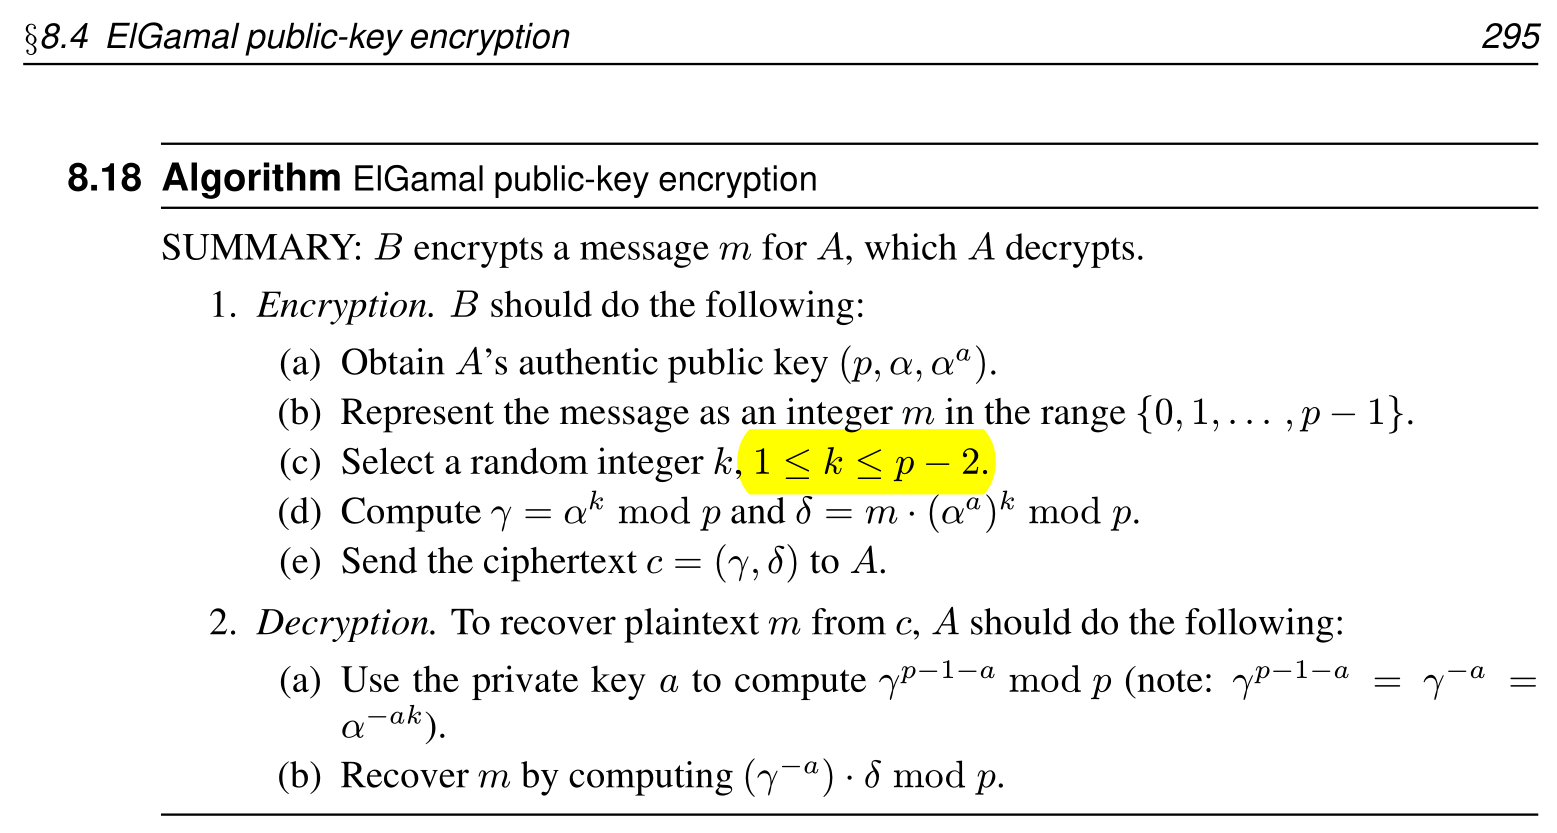
\includegraphics[width=.5\textwidth]{hac-enc}};
    \node at (0,0) {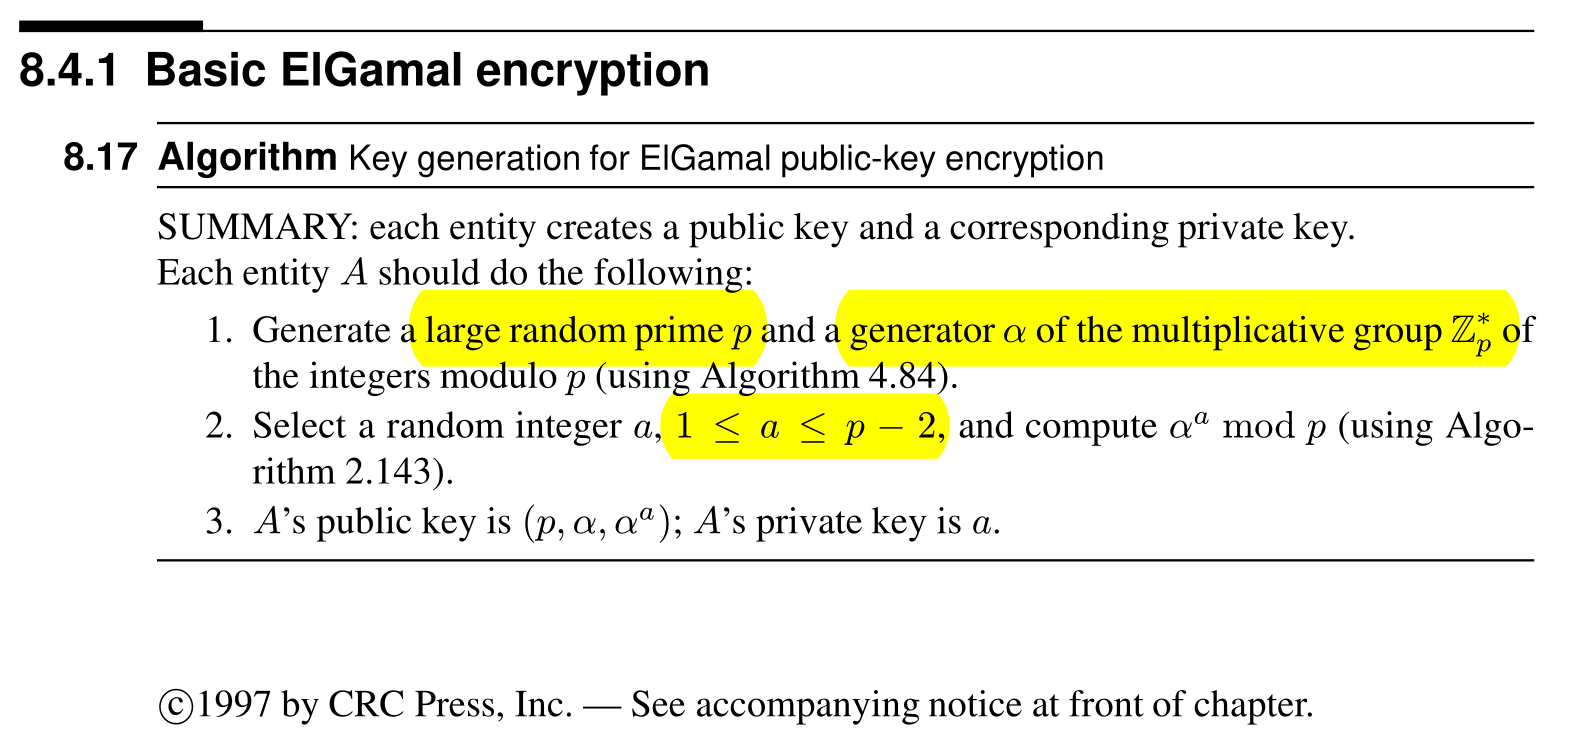
\includegraphics[width=.5\textwidth]{hac-gen}};
    \node at (5,-0.5) {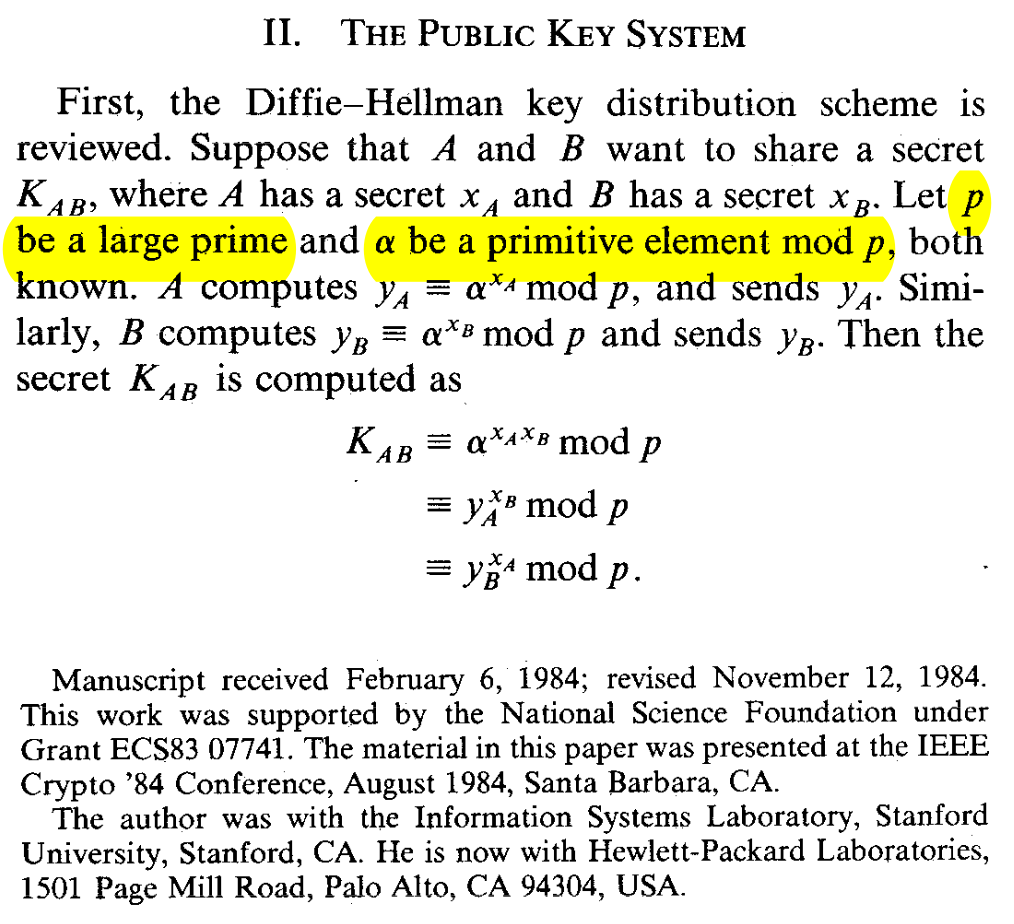
\includegraphics[width=.35\textwidth]{elgamal-gen}};
    \node at (5.4,-4) {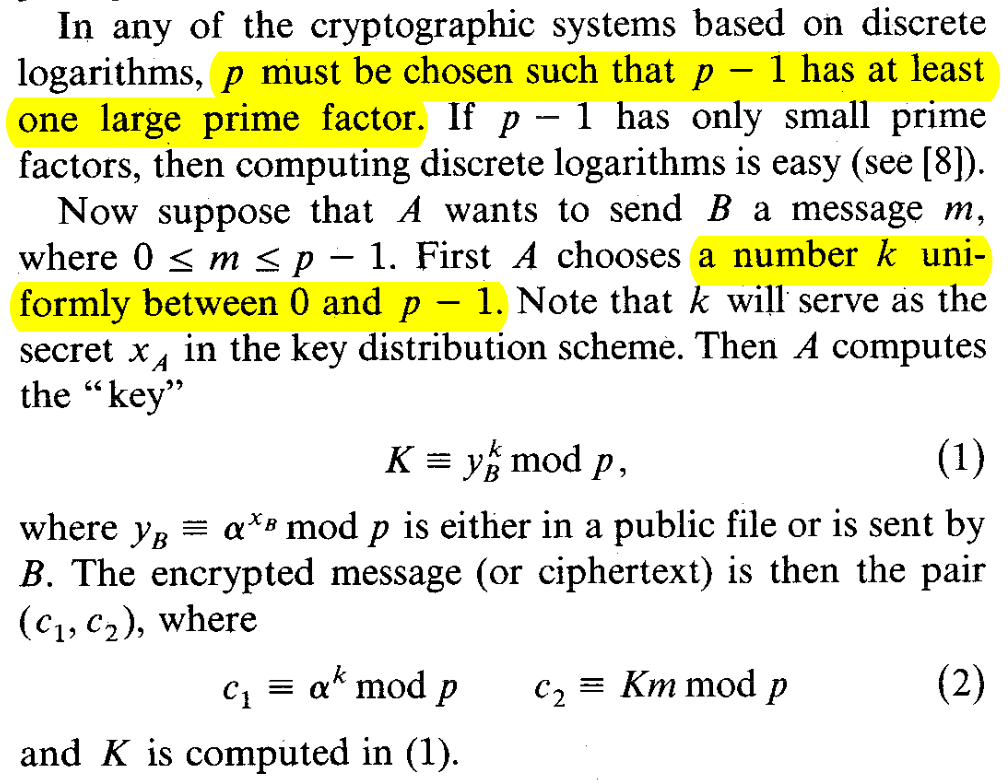
\includegraphics[width=.35\textwidth]{elgamal-enc}};
  \end{tikzpicture}
\end{frame}

%%

\begin{frame}{ElGamal in the wild (OpenPGP ecosystem)}
  \large
  \begin{description}[leftmargin=8cm]
    \setlength{\itemsep}{2em}
  \item[Large prime $p$] \hfill Safe prime \hfill ``Schnorr'' prime
    \hfill ``Lim-Lee'' prime \hfill other \hfill\strut
  \item[Generator $\alpha$] \hfill primitive element \hfill generates
    subgroup \hfill\strut
  \item[Private key] \hfill $0 < a < p$ \hfill ``short exponent'' optimisation \hfill\strut
  \item[Ephemeral key] \hfill $0 < k < p$ \hfill ``short exponent'' optimisation \hfill\strut
  \end{description}
\end{frame}

%%

\begin{frame}{What could possibly go wrong?}
  \centering
  \begin{tikzpicture}[x=.1\textwidth]
    \node at (0,0) {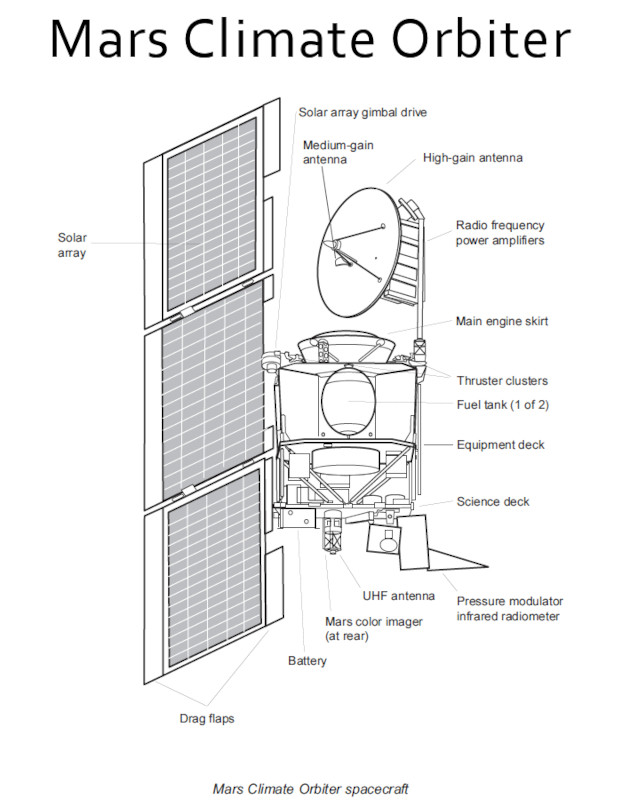
\includegraphics[height=.9\textheight]{mars}};
    \node at (-5,0) {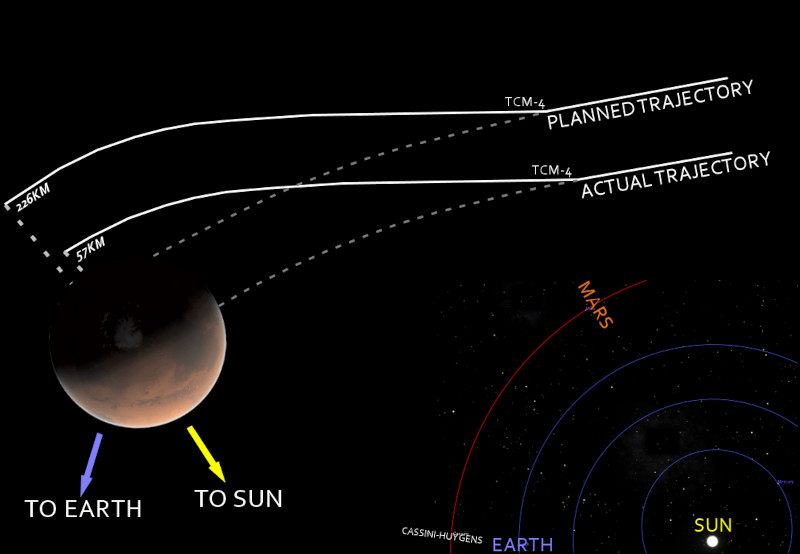
\includegraphics[width=.5\textwidth]{mars-orbit}};
    \node at (-7,-3.5) {\tiny credit: Wikipedia};
  \end{tikzpicture}
\end{frame}

%%

\begin{frame}{Our results}
  \begin{itemize}
    \setlength{\itemsep}{1em}
  \item<1-> Each of \emph{GPG}, \emph{Botan} and \emph{Libcrypto++}
    implements ElGamal in a different, non-RFC-4880-compliant way:
    \begin{itemize}
    \item Each is \emph{secure taken in isolation}.
    \item They are interoperable: functionally and securely.
    \end{itemize}
  \item<3-> We analyse 800K registered PGP ElGamal public keys:
    \begin{itemize}
    \item 40K of them are not consistent with any key
      generation algorithm we found in open source libraries.
    \item 2K of them are exposed to \emph{practical plaintext
        recovery} when \emph{GPG}, \emph{Botan}, \emph{Libcrypto++}
      (or any other library using the ``short exponent'' optimisation)
      \emph{encrypts to them}.\\
      We call these \emph{cross-configuration} attacks.
    \end{itemize}
  \item<2-> \emph{Go} does not implement ElGamal key generation and is \emph{the
    least offender}.
  \item<4-> We find side channels leaking ElGamal secret keys in \emph{GPG}, \emph{Go} and
    \emph{Libcrypto++}:
    \begin{itemize}
    \item \emph{GPG} claimed to be side-channel resistant.
    \item Our attack against \emph{GPG} becomes more powerful in the
      \emph{cross-configuration} scenario.
    \end{itemize}
  \end{itemize}
\end{frame}

%%

\begin{frame}{Why a large prime factor, anyway?}
  \[\exp_\alpha \;:\; x \,\mapsto\, \alpha^x \mod p\]
  \emph{Discrete Logarithm Problem (DLP):} find $x$

  \begin{block}{Pohlig--Hellman algorithm \small(Chinese remainder theorem)}
    \centering
    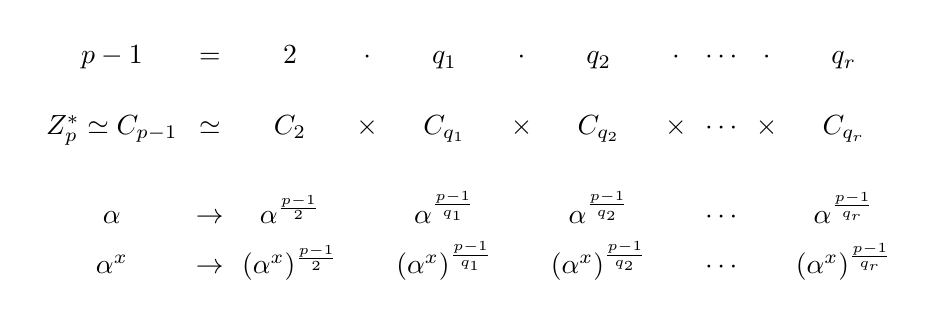
\begin{tikzpicture}[ampersand replacement=\&]
      \matrix (m) [matrix of math nodes] {
        p-1 \& = \& 2 \& \cdot \& q_1 \& \cdot \& q_2 \& \cdot \& \cdots \& \cdot \& q_r\\[1em]
        \Z_p^* \simeq C_{p-1} \& \simeq \& C_2 \& \times \& C_{q_1} \& \times \& C_{q_2} \& \times \& \cdots \& \times \& C_{q_r}\\[1em]
        \alpha \& \to \& \alpha^{\frac{p-1}{2}} \& \& \alpha^{\frac{p-1}{q_1}} \& \& \alpha^{\frac{p-1}{q_2}} \& \& \cdots \& \& \alpha^{\frac{p-1}{q_r}}\\
        \alpha^x \& \to \& (\alpha^x)^{\frac{p-1}{2}} \& \& (\alpha^x)^{\frac{p-1}{q_1}} \& \& (\alpha^x)^{\frac{p-1}{q_2}} \& \& \cdots \& \& (\alpha^x)^{\frac{p-1}{q_r}}\\
      };
    \end{tikzpicture}
  \end{block}

  Cost to solve DLP in \emph{$C_{q_i}$} is \emph{$O(\sqrt{q_i})$}.
\end{frame}

%%

\begin{frame}{Concretely (FIPS 186-2)}
  \Large\centering
  \begin{tabular}{c@{\hspace{1cm}}c@{\hspace{1cm}}c}
    bitlength of $p$ & bitlength of largest $q|(p-1)$ & security (bits)\\
    \hline
    1024 & 160 & 80\\
    2048 & 224 & 112\\
    3072 & 256 & 128\\
    7680 & 384 & 192\\
    15360 & 512 & 256
  \end{tabular}
\end{frame}

%%

\begin{frame}{Prime generation}
  \begin{description}[labelwidth=0,leftmargin=!]
    \setlength{\itemsep}{1em}
  \item[Goal:] prime $p$ with at least \emph{one large prime factor $q|(p-1)$}.
  \item[Safe primes:] $p = 2\emph{q} + 1$:
    \begin{itemize}
    \item Considered kind of expensive, back in the '90s.
    \end{itemize}
  \item[``Lim-Lee'' primes:] $p = 2\emph{q_1}q_2\cdots q_r$, all $q_i$ large:
    \begin{itemize}
    \item Cheaper than safe primes,
    \item Protecting against the same \emph{attacks}.
    \end{itemize}
  \item[``Schnorr'' primes:] $p = 2\emph{q}f + 1$, with $f$ arbitrary:
    \begin{itemize}
    \item Cheapest,
    \item Popularized by Schnorr signatures, DSA, FIPS-186-2.
    \end{itemize}
  \item[Random primes:] risky, don't do it!
  \item[Other:] your imagination is the only limitation!
  \end{description}
\end{frame}

%%

\begin{frame}{Solving DLP with ``short'' exponents (van Oorschot--Wiener '96)}
  \begin{block}{}
    \centering
    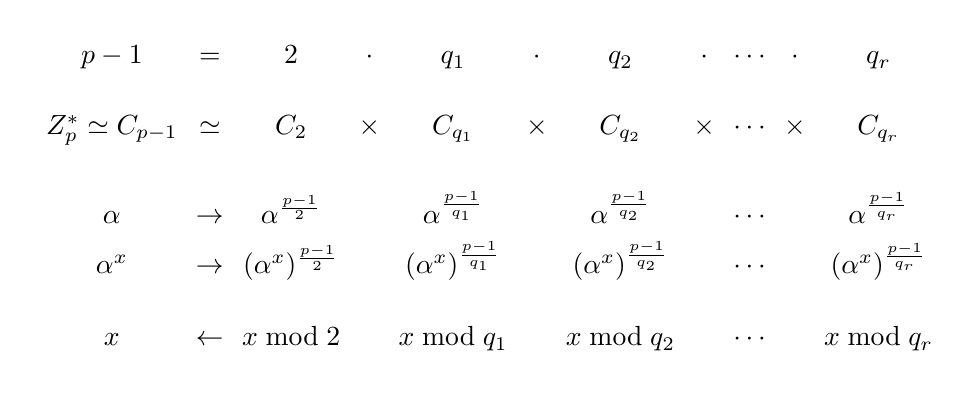
\begin{tikzpicture}[ampersand replacement=\&]
      \matrix (m) [matrix of math nodes] {
        p-1 \& = \& 2 \& \cdot \& q_1 \& \cdot \& q_2 \& \cdot \& \cdots \& \cdot \& q_r\\[1em]
        \Z_p^* \simeq C_{p-1} \& \simeq \& C_2 \& \times \& C_{q_1} \& \times \& C_{q_2} \& \times \& \cdots \& \times \& C_{q_r}\\[1em]
        \alpha \& \to \& \alpha^{\frac{p-1}{2}} \& \& \alpha^{\frac{p-1}{q_1}} \& \& \alpha^{\frac{p-1}{q_2}} \& \& \cdots \& \& \alpha^{\frac{p-1}{q_r}}\\
        \alpha^x \& \to \& (\alpha^x)^{\frac{p-1}{2}} \& \& (\alpha^x)^{\frac{p-1}{q_1}} \& \& (\alpha^x)^{\frac{p-1}{q_2}} \& \& \cdots \& \& (\alpha^x)^{\frac{p-1}{q_r}}\\[1em]
        x \& \gets \& x\bmod 2 \& \& x\bmod q_1 \& \& x\bmod q_2 \& \& \cdots \& \& x\bmod q_r\\
      };
    \end{tikzpicture}
  \end{block}

  \bigskip
  
  Suppose \emph{$\log(x) < \log(q_1) + \log(q_2) + \log(q_3)$} $\Rightarrow$
  We \emph{don't need} to solve for \emph{$x\bmod q_4$}, \dots
\end{frame}

%%

\begin{frame}{The group generator}
  \begin{block}{Primitive element}
    $\alpha\in\Z_p^*$ is a \emph{primitive element} if every element 
    $\beta\in\Z_p\setminus\{0\}$ can be written (uniquely) as
    \[\beta = \alpha^x \qquad\qquad 0\le x < p-1.\]
  \end{block}

  \begin{block}{Prime order subgroup generator}
    $\alpha\ne 0,1$ \emph{generates the subgroup} $G\subset\Z_p^*$
    of prime order $q$ if
    \[\alpha^q = 1.\]
  \end{block}

  \begin{itemize}
  \item Both El Gamal and {\it the Handbook} mandate a primitive
    element $\alpha$.
  \item Modern practice recommends a generator of a
    subgroup of large prime order $q$
    \begin{description}
    \item[Example:] if $p = 2q + 1$ is a safe prime, $4$ 
      always generates the subgroup of order $q$.
    \item[Bonus:] protects against Pohlig--Hellman attacks, and more.
    \end{description}
  \end{itemize}
\end{frame}

%%

\begin{frame}{ElGamal Encryption \uncover<7->{in OpenPGP}}
  \begin{tikzpicture}
    \begin{uncoverenv}<1-4>
      \begin{scope}
        \large
        \node at (0,0) {$p$};
        \node at (0,-.7) {$\alpha \bmod p$};
        \node at (0,-1.4) {$\alpha^x = X$};
      \end{scope}
      \begin{scope}[anchor=west,xshift=1.5cm,color=black!60]
        \node at (0,0) {prime};
        \node at (0,-.7) {generator};
        \node at (0,-1.4) {public key};
      \end{scope}
    \end{uncoverenv}
    
    \begin{uncoverenv}<2-4>
      \begin{scope}[xshift=11cm]
        \large
        \node at (0,0) {$m$};
        \node at (0,-.7) {$y$};
      \end{scope}
      \begin{scope}[xshift=12.5cm,color=black!60]
        \node at (0,0) {message};
        \node at (0,-.7) {random};
      \end{scope}
    \end{uncoverenv}
    
    \begin{uncoverenv}<3>
      \begin{scope}[xshift=6cm,yshift=-3.5cm]
        \Large
        \node at (0,0) {$(Y=\alert{\alpha^y},\quad X^y\cdot m)$};
        \node at (0,-1.5) {$m = X^y\cdot m / \alert{Y^x}$};
      \end{scope}
      \begin{scope}[xshift=10cm,yshift=-3.5cm,color=black!60]
        \node at (0,0) {encryption};
        \node at (0,-1.5) {decryption};
      \end{scope}
    \end{uncoverenv}

    \begin{uncoverenv}<4->
      \begin{scope}[yshift=-3cm]
        \large
        \node at (0,0) {$(p-1) = $};
        \node at (0,-1) {$\alpha$};
        \node at (0,-2) {$x\in$};
        \node at (0,-3) {$y\in$};
        \uncover<10->{
          \node[scale=2] at (14.1,-1) {$\Biggr\}$};
          \node[scale=2] at (14.1,-3) {$\}$};
        }
      \end{scope}
      \begin{scope}[anchor=west,xshift=1.5cm,yshift=-3cm]
        \begin{scope}[gray,yshift=0.4cm]
          \scriptsize
          \node at (0.1,0) {safe};
          \node at (2.1,0) {Schnorr};
          \node at (5.6,0) {Lim-Lee};
        \end{scope}
        \node at (0,0) {$2\cdot q$};
        \node at (2,0) {$2\cdot f \cdot q$};
        \node at (5,0) {$2\cdot q \cdot q_2 \cdots q_r$};
        \node at (0,-1) {generates all of $\Z_p^*$};
        \node at (4,-1) {generates subgroup of order $q$};
        \node at (1,-2) {$[1,p-1]$};
        \node at (5,-2) {``short''};
        \node at (1,-3) {$[1,p-1]$};
        \node at (5,-3) {``short''};
        %% 
        \uncover<5->{\draw[thick,blue] (2.6,-.2) -- (1.8,-.8) (1.8,-1.2) -- (5.5,-1.8);}
        \uncover<6->{\draw[thick,red] (2.5,-.2) -- (1.7,-.8) (1.7,-1.2) -- (5.5,-2.8);}
      \end{scope}
      \begin{scope}[anchor=east,xshift=14cm,yshift=-3cm,color=black!60]
        \small
        \node at (0,0) {($q$ are ``large'' primes)};
        \node at (0,-1) {(other possible)};
      \end{scope}
    \end{uncoverenv}

    \begin{uncoverenv}<5-6>
      \begin{scope}[anchor=east,xshift=4cm,yshift=-.5cm]
        \node[color=blue] at (0,0) {Bingo 0:};
        \uncover<6->{
          \node[color=red] at (0,-.7) {Bingo 1:};
        }
      \end{scope}
      \begin{scope}[anchor=west,xshift=4.5cm,yshift=-.5cm]
        \node at (0,0) {key recovery from public key only (van Oorschot--Wiener)};
        \uncover<6->{
          \node at (0,-.7) {message recovery from single ciphertext (this work)};
        }
      \end{scope}
    \end{uncoverenv}

    \begin{uncoverenv}<7->
      \begin{scope}[anchor=west,yshift=.5cm]
        \uncover<7->{
          \node at (0,-.7) {\textcolor{green!80!black}{\texttt{libgcrypt}:} Lim-Lee, generates all $\Z_p^*$, short exponents.};
        }
        \uncover<8->{
          \node at (0,-1.4) {\textcolor{purple}{\texttt{libcrypto++}:} safe primes, generates subgroup, short exponents.};
        }
        \uncover<9->{
          \node at (0,-2.1) {\texttt{Go:} no key generation, $y\in[1,p-1]$.};
        }
      \end{scope}
      \begin{scope}[xshift=1.5cm,yshift=-3cm,dashed]
        \uncover<7->{
          \draw[green!80!black] (6,-.2) -- (1.9,-.8) (2.1,-1.2) -- (5.8,-1.8) (5.8,-2.2) -- (5.8,-2.8);
        }
        \uncover<8->{
          \draw[purple] (1,-.2) -- (6,-.8) (6,-1.2) -- (6,-1.8) (6,-2.2) -- (6,-2.8);
          }
      \end{scope}
    \end{uncoverenv}
  \end{tikzpicture}
  \vspace{1cm}
\end{frame}

%%

\begin{frame}{OpenPGP implementations}
  \large
  \begin{center}
  \fcolorbox{gray}{cyan!10}{%
    \begin{minipage}{11cm}%
      \begin{tabular}{ll}
        \textbf{libgcrypt} & $\bullet$ backbone of GnuPG; ElGamal code from 1997 \\
                           & $\bullet$ Lim--Lee primes, full group, short-ish exponents \medskip \\
        \textbf{Crypto++}  & $\bullet$ ElGamal code from 2002 \\
                           & $\bullet$ safe primes, almost full group, short exponents \medskip \\
        \textbf{Golang}    & $\bullet$ no key generation, long exponents\\
      \end{tabular}%
    \end{minipage}%
  }

  \bigskip

  \fcolorbox{gray}{cyan!10}{%
    \begin{minipage}{11cm}%
      \begin{tabular}{l@{\qquad}c@{\qquad}c@{\qquad}c@{\qquad}c@{\qquad}c}
        & $\lvert p \rvert$ & $\lvert q \rvert$ & $\lvert x \rvert$ & $\lvert y \rvert$ & $\langle \alpha\rangle$ \\
        \textbf{libgcrypt} & 2048 & 225 & 344 & \alert<2>{344} & $\Z_p^*$ \\
        \textbf{Crypto++}  & 2048 & 2047 & 226 & \alert<2>{226} & $\mathsf{QR}(p)$ \\
        \textbf{Golang}    & 2048 & - & - & 2048 & -  \\
      \end{tabular}%
    \end{minipage}%
  }

  \medskip
  For any two, generating keys with the one and encrypting with the other is secure
\end{center}
\end{frame}

%%

\begin{frame}{OpenPGP ElGamal keys in the wild (Jan 2021)}
  \large
  \begin{center}
  \fcolorbox{gray}{cyan!10}{%
    \begin{tabular}{l|ccc|r|r}
    \multicolumn{1}{c}{prime type} & \multicolumn{3}{c}{group size} & \multicolumn{2}{c}{quantity} \\
    & $p-1$ & $q$ & other & total & since 2016 \\
    Safe prime I   & x & & & 472,518 & 783 \\
    Safe prime II  & & x & & 107,339 & 219 \\
    Lim--Lee I      & ? & & & 211,271 & 6003 \\
    Lim--Lee II     & & ? & & 47 & 24 \\
    % Quasi-safe I   & x & & & 15,592 & 89 \\
    % Quasi-safe II  & & x & & 20 & 3 \\
    % Quasi-safe III & & & x & 26,199 & 125 \\
    \only<1>{%
    Schnorr I     & ? & & & 828 & 810 \\
    Schnorr II    & & ? & & 27 & 26 \\
    Schnorr III   & & & x & 1,304 & 1300
    }%
    \only<2>{%
    \color{red}Schnorr I     & \color{red}? & & & 828 & 810 \\
    Schnorr II    & & ? & & 27 & 26 \\
    \color{red}Schnorr III   & & & \color{red}x & 1,304 & 1300
    }%
    \end{tabular}%
  }\\
  \strut 2.7M keys in total, 800k out of which were ElGamal
  \end{center}
\end{frame}

%%

\begin{frame}{Side channel vulnerabilities in exponentiation}
  \begin{description}
  \item[Goal] Key recovery.
  \item[Threat model]
    \begin{itemize}
    \item Co-located attacker;
    \item Targets the exponentiation in the decryption routine;
    \item Must trigger decryption (e.g., email decryption).
    \end{itemize}
  \item[Techniques] FLUSH+RELOAD (instruction cache), PRIME+PROBE (data cache).
  \item[Findings]\
    
    \begin{tabular}{l | c c c }
      \backslashbox{Key}{Library} & \texttt{libcrypto++} & \texttt{Go} & \texttt{libgcrypt}\\
      \hline
      $x\in[1,p-1]$ & $|$ & $|$ & unfeasible\\
      \texttt{libgcrypt} & trivial & easy & unfeasible/state\\
      \texttt{libcrypto++} & $|$ & $|$ & state/commodity*\\
    \end{tabular}
  \end{description}

  \bigskip
  *Verified experimentally on 2048 bits key.  
\end{frame}

%%

\begin{frame}{Our results}
  \begin{itemize}
    \setlength{\itemsep}{1em}
  \item Each of \emph{GPG}, \emph{Botan} and \emph{Libcrypto++}
    implements ElGamal in a different, non-RFC-4880-compliant way:
    \begin{itemize}
    \item Each is \emph{secure taken in isolation}.
    \item They are interoperable: functionally and securely.
    \end{itemize}
  \item We analyse 800K registered PGP ElGamal public keys:
    \begin{itemize}
    \item 40K of them are not consistent with any key
      generation algorithm we found in open source libraries.
    \item 2K of them are exposed to \emph{practical plaintext
        recovery} when \emph{GPG}, \emph{Botan}, \emph{Libcrypto++}
      (or any other library using the ``short exponent'' optimisation)
      \emph{encrypts to them}.\\
      We call these \emph{cross-configuration} attacks.
    \end{itemize}
  \item \emph{Go} does not implement ElGamal key generation and is \emph{the
    least offender}.
  \item We find side channels leaking ElGamal secret keys in \emph{GPG}, \emph{Go} and
    \emph{Libcrypto++}:
    \begin{itemize}
    \item \emph{GPG} claimed to be side-channel resistant.
    \item Our attack against \emph{GPG} becomes more powerful in the
      \emph{cross-configuration} scenario.
    \end{itemize}
  \end{itemize}
\end{frame}

\end{document}


% LocalWords:  Isogeny abelian isogenies hyperelliptic supersingular Frobenius
% LocalWords:  isogenous
